% Dans l'introduction, on présente le problème étudié et les buts
% poursuivis. L'introduction permet de faire connaître le cadre de la
% recherche et d'en préciser le domaine d'application. Elle fournit
% les précisions nécessaires en ce qui concerne le contexte de
% réalisation de la recherche, l'approche envisagée, l'évolution de
% la réalisation. En fait, l'introduction présente au lecteur ce
% qu'il doit savoir pour comprendre la recherche et en connaître la
% portée.
\Chapter{INTRODUCTION}\label{sec:Introduction}  % 10-12 lignes pour introduire le sujet.

%%
%%  Contexte et problématique
%%

\section{Contexte et problématique}

La valeur du marché des solutions \texttt{ERP} s'établissait autour de 40 milliards \texttt{USD} mondialement en 2020 \cite{mordorintelligence_erp_2023,bigbang_erp_2023}. Le coût moyen par utilisateur, sur 5 ans, s'élevait à 9 000\$, pour une \texttt{PME}, en 2022 \cite{softwarepath_erp_2023}.

Le développement de système \texttt{ERP} est complexe, nécessite une maintenance exigeante et le risque d’introduire des erreurs est important. Comment accélérer le développement de fonctionnalités de la plateforme \texttt{ERP} \texttt{Odoo} 12 communautaire?

La plateforme \texttt{ERPLibre} a été créée dans l’objectif d’accélérer le développement de la plateforme \texttt{Odoo} 12 communautaire. Ce mémoire va mettre l’accent sur la génération de code par des techniques de rétro-ingénierie et la gestion d’une communauté dans un contexte d’un projet logiciel libre.

% TODO point de départ : «Code projet initial générateur de code» et donner REF

% Projet morceau de l'automate, son fondement libre, par sa création de technopoïèse.
% Il utiliser pour la liberté de l'automate d’offrir librement accès à ses fonctionnalités
% Il étudier comprendre et accepter son fonctionnement
% Il copier pour se l’approprier en respectant le copyright
% Il modifier son amélioration en tant que développement logiciel

% Combien ça prend de temps pour développer la migration pour autant de fonctionnalités? Ajouter des champs, migrer des champs en changeant leur nature.

\subsection{Choix de la plateforme \texttt{ERP}}

Choisir une plateforme \texttt{ERP} libre peut offrir des avantages significatifs en termes de coût, de flexibilité, de sécurité, de communauté et d'indépendance. \texttt{Odoo} a été choisi puisqu'il répondait à ces critères, cependant quelle est la version qui offre le plus de fonctionnalité?

\begin{table}
\caption{Tableau des dates de lancement du logiciel \texttt{Odoo}}
\centering
\begin{tabular}{|c|c|l|l|}

\hline
Légende & \cellcolor[HTML]{d9ead3}{\shortstack[l]{Version actuelle}} & \cellcolor[HTML]{fff2cc}{\shortstack[l]{Anciennes versions avec \\ maintenance étendu}} & \cellcolor[HTML]{f4cccc}{\shortstack[l]{Anciennes versions ou \\ fin de maintenance}}\\\hline

\hline\rowcolor[gray]{0.8}\color{black}
\texttt{Odoo} version & Date de lancement & \multicolumn{2}{|l|}{Commentaire}\\\hline
\cellcolor[HTML]{f4cccc}6.0/6.1 & octobre 2009 & \multicolumn{2}{|l|}{Première publication sous \texttt{AGPL}, premier client web}\\\hline
\cellcolor[HTML]{f4cccc}7.0 & décembre 2012 & \multicolumn{2}{|l|}{} \\\hline
\cellcolor[HTML]{f4cccc}8.0 & septembre 2014 & \multicolumn{2}{|l|}{\shortstack[l]{Changement de nom pour \texttt{Odoo}, anciennement \\ \texttt{OpenERP}}}\\\hline
\cellcolor[HTML]{f4cccc}9.0 & novembre 2015 & \multicolumn{2}{|l|}{\shortstack[l]{Première publication des éditions \texttt{Community} sous \\ licence \texttt{LGPLV3} et \texttt{Enterprise} sous licence \\ propriétaire.}}\\\hline
\cellcolor[HTML]{f4cccc}10.0 & octobre 2016 & \multicolumn{2}{|l|}{} \\\hline
\cellcolor[HTML]{f4cccc}11.0 & octobre 2017 & \multicolumn{2}{|l|}{} \\\hline
\cellcolor[HTML]{f4cccc}12.0 & octobre 2018 & \multicolumn{2}{|l|}{Version utilisé dans \texttt{ERPLibre} 1.5.0}\\\hline
\cellcolor[HTML]{fff2cc}13.0 & octobre 2019 & \multicolumn{2}{|l|}{}\\\hline
\cellcolor[HTML]{fff2cc}14.0 & octobre 2020 & \multicolumn{2}{|l|}{} \\\hline
\cellcolor[HTML]{fff2cc}15.0 & octobre 2021 & \multicolumn{2}{|l|}{} \\\hline
\cellcolor[HTML]{d9ead3}16.0 & octobre 2022 & \multicolumn{2}{|l|}{} \\\hline
\end{tabular}
\label{tab:choix_plateform_erp}
\end{table}

% Regarder l’évolution des modules dans \texttt{OCA}, en prenant leur nom de module, pour chaque version d’\texttt{Odoo}, selon une date déterminée, regarder le nombre de fois qu’il se répète. Ceci va indiquer la vitesse de migration des modules dans la communauté.

En janvier 2023, les versions 9.0 à 12.0 ne sont plus supportées officiellement par la compagnie \texttt{Odoo}, voir tableau \ref{tab:choix_plateform_erp}, mais elles le sont encore par \texttt{OCA}. La version 16.0 est la version stable actuelle. La démonstration commence à partir de 9.0, là où débute la divergence entre une version communautaire et entreprise.

Au printemps 2020, \texttt{Odoo} version 12.0 a été choisi par \texttt{ERPLibre}\footnote{Première version de \texttt{ERPLibre} : \url{https://github.com/ERPLibre/ERPLibre/releases/tag/v0.1.0}.}. Une recherche de module par version d'\texttt{Odoo} a été effectué sur 11 Go de code et de données sur le projet \texttt{ERPLibre} version 1.5.0, voir le tableau \ref{tab:nb_module_version_odoo}. Ainsi, en date du 1 janvier 2023, la version 12.0 est encore le bon choix avec 2 977 modules, puisqu'il est celui qu'il a le plus de module sur les 133 répertoires gérés par \texttt{ERPLibre}. Cette tendance pourrait changer en 2024 selon l’évolution.

Pour obtenir les résultats du tableau \ref{tab:nb_module_version_odoo}, un script a été développé pour chercher la quantité de modules en cherchant dans les 133 répertoires \texttt{Git}, puis pour toutes les versions d'\texttt{Odoo}, pour tous les modules qui contiennent le fichier «manifest» et que ceux-ci inclus le paramètre qu'il est installable, à date précédente du 1 janvier de chaque année.
% le fichier «\_\_openerp\_\_.py» ou «\_\_manifest\_\_.py»

Des fois, la quantité de module diminue d'une année à l'autre. Il y a création d'une nouvelle branche lors d'une nouvelle version qui est la suite de la version précédente. Par exemple, dans le tableau \ref{tab:nb_module_version_odoo}, la version 10.0 entre 2017 et 2018, il y a une réduction de 171 modules dans les répertoires d'entreprise, mais il y a eu seulement 4 mois pour faire le nettoyage, les méthodes de mises à jours ont évolués depuis.

De plus, les chiffres du tableau \ref{tab:nb_module_version_odoo} semblent démontrer que les versions paires d'\texttt{Odoo} sont plus populaire que les versions impaires. Cependant la communauté d'\texttt{Odoo} est bien plus grosse que 133 répertoires.

Dans la section total du tableau \ref{tab:nb_module_version_odoo}, la section unique signifie que la somme va ignorer les doublons. En date du 1 janvier 2023, il y a au total 17 309 modules, mais 6 063 modules uniques. Ça signifie qu'il y a 11 246 modules en doublon. Hors, le code diffère d'une version à l'autre même si c'est un doublon, ils peuvent avoir des bogues ou des fonctionnalités différentes entre eux.

% Prochain tableau
\begin{table}
\caption{Nombre de modules par version \texttt{Odoo} à partir du 1 janvier minuit par année sur la plateforme \texttt{ERPLibre} 1.5.0.}
\centering
\begin{tabular}{|l|l|l|l|l|l|l|l|l|}
\hline

Légende & \multicolumn{2}{|l|}{\shortstack[l]{Total\\\textcolor[HTML]{274e13}{OCA}\\\textcolor[HTML]{4c1130}{Entreprise}}} & \multicolumn{2}{|c|}{\cellcolor[HTML]{d9ead3}{\shortstack[l]{Version \\ actuelle}}} & \multicolumn{2}{|c|}{\cellcolor[HTML]{fff2cc}{\shortstack[l]{Anciennes \\ versions avec \\ maintenance \\ étendu}}} & \multicolumn{2}{|c|}{\cellcolor[HTML]{f4cccc}{\shortstack[l]{Anciennes \\ versions ou \\ fin de \\ maintenance}}}\\\hline

\multicolumn{9}{|l|}{\shortstack[l]{17309/\textcolor[HTML]{274e13}{10728}/\textcolor[HTML]{4c1130}{6581} modules à supporter le 1 janvier 2023 \\ 17465/\textcolor[HTML]{274e13}{10952}/\textcolor[HTML]{4c1130}{6513} modules le 15 février 2023 \\ 156/\textcolor[HTML]{274e13}{132}/\textcolor[HTML]{4c1130}{24} nouveaux modules en 31 jours durant janvier 2023}}\\\hline

\texttt{Odoo} version & 2016 & 2017 & 2018 & 2019 & 2020 & 2021 & 2022 & 2023 \\\hline

6.1 &
\cellcolor[HTML]{fff2cc}{\shortstack[r]{295 \\ \textcolor[HTML]{274e13}{269} \\ \textcolor[HTML]{4c1130}{26}}} & 
\cellcolor[HTML]{f4cccc}{\shortstack[r]{299 \\ \textcolor[HTML]{274e13}{270} \\ \textcolor[HTML]{4c1130}{29}}} &
\cellcolor[HTML]{f4cccc}{\shortstack[r]{299 \\ \textcolor[HTML]{274e13}{270} \\ \textcolor[HTML]{4c1130}{29}}} &
\cellcolor[HTML]{f4cccc}{\shortstack[r]{299 \\ \textcolor[HTML]{274e13}{270} \\ \textcolor[HTML]{4c1130}{36}}} &
\cellcolor[HTML]{f4cccc}{\shortstack[r]{299 \\ \textcolor[HTML]{274e13}{270} \\ \textcolor[HTML]{4c1130}{36}}} &
\cellcolor[HTML]{f4cccc}{\shortstack[r]{299 \\ \textcolor[HTML]{274e13}{270} \\ \textcolor[HTML]{4c1130}{36}}} &
\cellcolor[HTML]{f4cccc}{\shortstack[r]{299 \\ \textcolor[HTML]{274e13}{270} \\ \textcolor[HTML]{4c1130}{36}}} &
\cellcolor[HTML]{f4cccc}{\shortstack[r]{299 \\ \textcolor[HTML]{274e13}{270} \\ \textcolor[HTML]{4c1130}{36}}} \\\hline

7.0 &
\cellcolor[HTML]{fff2cc}{\shortstack[r]{637 \\ \textcolor[HTML]{274e13}{597} \\ \textcolor[HTML]{4c1130}{40}}} & 
\cellcolor[HTML]{fff2cc}{\shortstack[r]{633 \\ \textcolor[HTML]{274e13}{592} \\ \textcolor[HTML]{4c1130}{41}}} &
\cellcolor[HTML]{f4cccc}{\shortstack[r]{634 \\ \textcolor[HTML]{274e13}{593} \\ \textcolor[HTML]{4c1130}{41}}} &
\cellcolor[HTML]{f4cccc}{\shortstack[r]{635 \\ \textcolor[HTML]{274e13}{594} \\ \textcolor[HTML]{4c1130}{41}}} &
\cellcolor[HTML]{f4cccc}{\shortstack[r]{669 \\ \textcolor[HTML]{274e13}{619} \\ \textcolor[HTML]{4c1130}{50}}} &
\cellcolor[HTML]{f4cccc}{\shortstack[r]{669 \\ \textcolor[HTML]{274e13}{619} \\ \textcolor[HTML]{4c1130}{50}}} &
\cellcolor[HTML]{f4cccc}{\shortstack[r]{669 \\ \textcolor[HTML]{274e13}{619} \\ \textcolor[HTML]{4c1130}{50}}} &
\cellcolor[HTML]{f4cccc}{\shortstack[r]{671 \\ \textcolor[HTML]{274e13}{619} \\ \textcolor[HTML]{4c1130}{52}}} \\\hline

8.0 &
\cellcolor[HTML]{fff2cc}{\shortstack[r]{741 \\ \textcolor[HTML]{274e13}{597} \\ \textcolor[HTML]{4c1130}{144}}} & 
\cellcolor[HTML]{fff2cc}{\shortstack[r]{1092 \\ \textcolor[HTML]{274e13}{907} \\ \textcolor[HTML]{4c1130}{185}}} &
\cellcolor[HTML]{fff2cc}{\shortstack[r]{1215 \\ \textcolor[HTML]{274e13}{996} \\ \textcolor[HTML]{4c1130}{219}}} &
\cellcolor[HTML]{f4cccc}{\shortstack[r]{1265 \\ \textcolor[HTML]{274e13}{1027} \\ \textcolor[HTML]{4c1130}{238}}} &
\cellcolor[HTML]{f4cccc}{\shortstack[r]{1290 \\ \textcolor[HTML]{274e13}{1036} \\ \textcolor[HTML]{4c1130}{254}}} &
\cellcolor[HTML]{f4cccc}{\shortstack[r]{1297 \\ \textcolor[HTML]{274e13}{1043} \\ \textcolor[HTML]{4c1130}{254}}} &
\cellcolor[HTML]{f4cccc}{\shortstack[r]{1340 \\ \textcolor[HTML]{274e13}{1049} \\ \textcolor[HTML]{4c1130}{291}}} &
\cellcolor[HTML]{f4cccc}{\shortstack[r]{1341 \\ \textcolor[HTML]{274e13}{1050} \\ \textcolor[HTML]{4c1130}{291}}} \\\hline

9.0 &
\cellcolor[HTML]{d9ead3}{\shortstack[r]{135 \\ \textcolor[HTML]{274e13}{46} \\ \textcolor[HTML]{4c1130}{89}}} & 
\cellcolor[HTML]{fff2cc}{\shortstack[r]{456 \\ \textcolor[HTML]{274e13}{346} \\ \textcolor[HTML]{4c1130}{110}}} &
\cellcolor[HTML]{fff2cc}{\shortstack[r]{725 \\ \textcolor[HTML]{274e13}{602} \\ \textcolor[HTML]{4c1130}{123}}} &
\cellcolor[HTML]{fff2cc}{\shortstack[r]{776 \\ \textcolor[HTML]{274e13}{643} \\ \textcolor[HTML]{4c1130}{133}}} &
\cellcolor[HTML]{f4cccc}{\shortstack[r]{796 \\ \textcolor[HTML]{274e13}{659} \\ \textcolor[HTML]{4c1130}{137}}} &
\cellcolor[HTML]{f4cccc}{\shortstack[r]{803 \\ \textcolor[HTML]{274e13}{666} \\ \textcolor[HTML]{4c1130}{137}}} &
\cellcolor[HTML]{f4cccc}{\shortstack[r]{844 \\ \textcolor[HTML]{274e13}{666} \\ \textcolor[HTML]{4c1130}{178}}} &
\cellcolor[HTML]{f4cccc}{\shortstack[r]{850 \\ \textcolor[HTML]{274e13}{669} \\ \textcolor[HTML]{4c1130}{181}}} \\\hline

10.0 &
\cellcolor[HTML]{cccccc}{} & 
\cellcolor[HTML]{d9ead3}{\shortstack[r]{523 \\ \textcolor[HTML]{274e13}{111} \\ \textcolor[HTML]{4c1130}{412}}} &
\cellcolor[HTML]{fff2cc}{\shortstack[r]{954 \\ \textcolor[HTML]{274e13}{713} \\ \textcolor[HTML]{4c1130}{241}}} &
\cellcolor[HTML]{fff2cc}{\shortstack[r]{1 537 \\ \textcolor[HTML]{274e13}{953} \\ \textcolor[HTML]{4c1130}{584}}} &
\cellcolor[HTML]{fff2cc}{\shortstack[r]{1 647 \\ \textcolor[HTML]{274e13}{1 047} \\ \textcolor[HTML]{4c1130}{600}}} &
\cellcolor[HTML]{f4cccc}{\shortstack[r]{1 685 \\ \textcolor[HTML]{274e13}{1 085} \\ \textcolor[HTML]{4c1130}{600}}} &
\cellcolor[HTML]{f4cccc}{\shortstack[r]{1 754 \\ \textcolor[HTML]{274e13}{1 109} \\ \textcolor[HTML]{4c1130}{645}}} &
\cellcolor[HTML]{f4cccc}{\shortstack[r]{1 765 \\ \textcolor[HTML]{274e13}{1 120} \\ \textcolor[HTML]{4c1130}{645}}} \\\hline

11.0 &
\cellcolor[HTML]{cccccc}{} & 
\cellcolor[HTML]{cccccc}{} &
\cellcolor[HTML]{d9ead3}{\shortstack[r]{288 \\ \textcolor[HTML]{274e13}{77} \\ \textcolor[HTML]{4c1130}{211}}} &
\cellcolor[HTML]{fff2cc}{\shortstack[r]{1 398 \\ \textcolor[HTML]{274e13}{658} \\ \textcolor[HTML]{4c1130}{740}}} &
\cellcolor[HTML]{fff2cc}{\shortstack[r]{1 710 \\ \textcolor[HTML]{274e13}{929} \\ \textcolor[HTML]{4c1130}{781}}} &
\cellcolor[HTML]{fff2cc}{\shortstack[r]{1 797 \\ \textcolor[HTML]{274e13}{1 000} \\ \textcolor[HTML]{4c1130}{797}}} &
\cellcolor[HTML]{f4cccc}{\shortstack[r]{1 860 \\ \textcolor[HTML]{274e13}{1 023} \\ \textcolor[HTML]{4c1130}{837}}} &
\cellcolor[HTML]{f4cccc}{\shortstack[r]{1 869 \\ \textcolor[HTML]{274e13}{1 032} \\ \textcolor[HTML]{4c1130}{864}}} \\

\noalign{\hrule height 2pt}
\multicolumn{1}{!{\vrule width 2pt}l!{\vrule width 1pt}}{\textbf{12.0}} &
\cellcolor[HTML]{cccccc}{} & 
\cellcolor[HTML]{cccccc}{} &
\cellcolor[HTML]{cccccc}{} &
\multicolumn{1}{!{\vrule width 2pt}r!{\vrule width 1pt}}{\textbf{\cellcolor[HTML]{d9ead3}{\shortstack[r]{784 \\ \textcolor[HTML]{274e13}{137} \\ \textcolor[HTML]{4c1130}{647}}}}} &
\multicolumn{1}{!{\vrule width 2pt}r!{\vrule width 1pt}}{\textbf{\cellcolor[HTML]{fff2cc}{\shortstack[r]{1 837 \\ \textcolor[HTML]{274e13}{993} \\ \textcolor[HTML]{4c1130}{844}}}}} &
\multicolumn{1}{!{\vrule width 2pt}r!{\vrule width 1pt}}{\textbf{\cellcolor[HTML]{fff2cc}{\shortstack[r]{2 503 \\ \textcolor[HTML]{274e13}{1 464} \\ \textcolor[HTML]{4c1130}{1 039}}}}} &
\multicolumn{1}{!{\vrule width 2pt}r!{\vrule width 1pt}}{\textbf{\cellcolor[HTML]{fff2cc}{\shortstack[r]{2 851 \\ \textcolor[HTML]{274e13}{1 633} \\ \textcolor[HTML]{4c1130}{1 218}}}}} &
\multicolumn{1}{!{\vrule width 2pt}r!{\vrule width 1pt}}{\textbf{\cellcolor[HTML]{f4cccc}{\shortstack[r]{2 977 \\ \textcolor[HTML]{274e13}{1 693} \\ \textcolor[HTML]{4c1130}{1 284}}}}} \\
\noalign{\hrule height 2pt}

13.0 &
\cellcolor[HTML]{cccccc}{} & 
\cellcolor[HTML]{cccccc}{} &
\cellcolor[HTML]{cccccc}{} &
\cellcolor[HTML]{cccccc}{} &
\cellcolor[HTML]{d9ead3}{\shortstack[r]{617 \\ \textcolor[HTML]{274e13}{115} \\ \textcolor[HTML]{4c1130}{502}}} &
\cellcolor[HTML]{fff2cc}{\shortstack[r]{1 445 \\ \textcolor[HTML]{274e13}{844} \\ \textcolor[HTML]{4c1130}{601}}} &
\cellcolor[HTML]{fff2cc}{\shortstack[r]{2 024 \\ \textcolor[HTML]{274e13}{1 310} \\ \textcolor[HTML]{4c1130}{714}}} &
\cellcolor[HTML]{fff2cc}{\shortstack[r]{2 241 \\ \textcolor[HTML]{274e13}{1 506} \\ \textcolor[HTML]{4c1130}{735}}} \\\hline

14.0 &
\cellcolor[HTML]{cccccc}{} & 
\cellcolor[HTML]{cccccc}{} &
\cellcolor[HTML]{cccccc}{} &
\cellcolor[HTML]{cccccc}{} &
\cellcolor[HTML]{cccccc}{} &
\cellcolor[HTML]{d9ead3}{\shortstack[r]{906 \\ \textcolor[HTML]{274e13}{129} \\ \textcolor[HTML]{4c1130}{777}}} &
\cellcolor[HTML]{fff2cc}{\shortstack[r]{2 150 \\ \textcolor[HTML]{274e13}{1 143} \\ \textcolor[HTML]{4c1130}{1 007}}} &
\cellcolor[HTML]{fff2cc}{\shortstack[r]{2 648 \\ \textcolor[HTML]{274e13}{1 698} \\ \textcolor[HTML]{4c1130}{950}}} \\\hline

15.0 &
\cellcolor[HTML]{cccccc}{} & 
\cellcolor[HTML]{cccccc}{} &
\cellcolor[HTML]{cccccc}{} &
\cellcolor[HTML]{cccccc}{} &
\cellcolor[HTML]{cccccc}{} &
\cellcolor[HTML]{cccccc}{} &
\cellcolor[HTML]{d9ead3}{\shortstack[r]{786 \\ \textcolor[HTML]{274e13}{96} \\ \textcolor[HTML]{4c1130}{690}}} &
\cellcolor[HTML]{fff2cc}{\shortstack[r]{1 669 \\ \textcolor[HTML]{274e13}{865} \\ \textcolor[HTML]{4c1130}{804}}} \\\hline

16.0 &
\cellcolor[HTML]{cccccc}{} & 
\cellcolor[HTML]{cccccc}{} &
\cellcolor[HTML]{cccccc}{} &
\cellcolor[HTML]{cccccc}{} &
\cellcolor[HTML]{cccccc}{} &
\cellcolor[HTML]{cccccc}{} &
\cellcolor[HTML]{cccccc}{} &
\cellcolor[HTML]{d9ead3}{\shortstack[l]{972 \\ \textcolor[HTML]{274e13}{206} \\ \textcolor[HTML]{4c1130}{766}}} \\\hline

\multicolumn{9}{|c|}{Total}\\\hline

Somme &
\shortstack[r]{1 808 \\ \textcolor[HTML]{274e13}{1 509} \\ \textcolor[HTML]{4c1130}{299}} & 
\shortstack[r]{3 003 \\ \textcolor[HTML]{274e13}{2 226} \\ \textcolor[HTML]{4c1130}{777}} &
\shortstack[r]{4 115 \\ \textcolor[HTML]{274e13}{3 251} \\ \textcolor[HTML]{4c1130}{864}} &
\shortstack[r]{6 701 \\ \textcolor[HTML]{274e13}{4 282} \\ \textcolor[HTML]{4c1130}{2 419}} &
\shortstack[r]{8 872 \\ \textcolor[HTML]{274e13}{5 668} \\ \textcolor[HTML]{4c1130}{3 204}} &
\shortstack[r]{11 411 \\ \textcolor[HTML]{274e13}{7 120} \\ \textcolor[HTML]{4c1130}{4 291}} &
\shortstack[r]{14 584 \\ \textcolor[HTML]{274e13}{8 918} \\ \textcolor[HTML]{4c1130}{5 666}} &
\shortstack[r]{17 309 \\ \textcolor[HTML]{274e13}{10 728} \\ \textcolor[HTML]{4c1130}{6 581}} \\\hline

Support \texttt{Odoo} &
\shortstack[r]{1 808 \\ \textcolor[HTML]{274e13}{1 509} \\ \textcolor[HTML]{4c1130}{299}} & 
\shortstack[r]{2 704 \\ \textcolor[HTML]{274e13}{1 956} \\ \textcolor[HTML]{4c1130}{748}} &
\shortstack[r]{3 182 \\ \textcolor[HTML]{274e13}{2 388} \\ \textcolor[HTML]{4c1130}{794}} &
\shortstack[r]{4 495 \\ \textcolor[HTML]{274e13}{2 391} \\ \textcolor[HTML]{4c1130}{2 104}} &
\shortstack[r]{5 811 \\ \textcolor[HTML]{274e13}{3 084} \\ \textcolor[HTML]{4c1130}{2 727}} &
\shortstack[r]{6 651 \\ \textcolor[HTML]{274e13}{3 437} \\ \textcolor[HTML]{4c1130}{3 214}} &
\shortstack[r]{7 811 \\ \textcolor[HTML]{274e13}{4 182} \\ \textcolor[HTML]{4c1130}{3 629}} &
\shortstack[r]{7 530 \\ \textcolor[HTML]{274e13}{4 275} \\ \textcolor[HTML]{4c1130}{3 255}} \\\hline

Unique &
\shortstack[r]{1 244 \\ \textcolor[HTML]{274e13}{1 047} \\ \textcolor[HTML]{4c1130}{197}} & 
\shortstack[r]{1 995 \\ \textcolor[HTML]{274e13}{1 435} \\ \textcolor[HTML]{4c1130}{560}} &
\shortstack[r]{2 260 \\ \textcolor[HTML]{274e13}{1 845} \\ \textcolor[HTML]{4c1130}{415}} &
\shortstack[r]{3 214 \\ \textcolor[HTML]{274e13}{2 172} \\ \textcolor[HTML]{4c1130}{1 042}} &
\shortstack[r]{3 927 \\ \textcolor[HTML]{274e13}{2 610} \\ \textcolor[HTML]{4c1130}{1 317}} &
\shortstack[r]{4 676 \\ \textcolor[HTML]{274e13}{3 080} \\ \textcolor[HTML]{4c1130}{1 596}} &
\shortstack[r]{5 452 \\ \textcolor[HTML]{274e13}{3 572} \\ \textcolor[HTML]{4c1130}{1 880}} &
\shortstack[r]{6 063 \\ \textcolor[HTML]{274e13}{3 980} \\ \textcolor[HTML]{4c1130}{2 083}} \\\hline

\multicolumn{9}{|l|}{\shortstack[l]{133/\textcolor[HTML]{274e13}{72}/\textcolor[HTML]{4c1130}{61} répertoires de modules dans \texttt{ERPLibre} 1.5.0}}\\\hline

\end{tabular}
\label{tab:nb_module_version_odoo}
\end{table}

\newpage
\subsection{Introduction Accorderie}

\subsection{Introduction Portail CEPPP}

\section{Définitions et concepts}

\subsection{Caractéristique de la plateforme Odoo}

\subsubsection{Internationalization et localisation}

\subsubsection{Architecture MVC}

\subsubsection{Website builder}

\subsubsection{Architecture ORM}

\subsubsection{Architecture modulaire par héritage}

\subsubsection{Fonctionnalité du hook lors de l’installation d’un module}

\subsubsection{ERPLibre}

\subsection{Communauté de développement}

\subsubsection{Générateur de code accessible dans la communauté Odoo}

\subsection{Cadre conceptuel}

\subsection{Exemples illustratifs d’Auto-reproducteur}

% \subsubsection{test}

% fds
% fds
% \paragraph{test2}

% fds
% fds

% \subparagraph{test3}


% fds

% Exemple
% Texte en \emph{italique}, \textsc{petites majuscules}, mot \mbox{insécable}.\\
% Texte \ul{souligné}, \hl{surligné}, \textbf{gras}.\\
% Texte entre ``guillemets''.\\
% Police \texttt{monospace}.\\
% Un mot courant en réseautique mobile: n\oe{}ud\footnote{Note de bas de page.}.\\
% L'objet RSVP \texttt{SENDER\_TEMPLATE}.\\
% Nom d'un auteur: \citeauthor{RFC_IPv4}.\\
% Une architecture 32~bits.\\
%%
%%  CONCEPTS DE BASE / BASIC CONCEPTS
%%
% \section{Définitions et concepts de base}  % environ 2-3 pages
% \begin{flushleft}
% 1\iere{} utilisation d'un acronyme yeah: \ac{IETF}.\\
% 2\ieme{} utilisation d'un acronyme: \ac{IETF}.\\ ça ne marche pas
% Acronyme au long: \acl{IETF}.\\
% \end{flushleft}

% \subsection{Une sous-section}
% Un URL: \href{http://www.polymtl.ca}{École Polytechnique de Montréal}.

% \subsubsection{Une sous-sous-section}
% Les besoins des flots de données peuvent être catégorisés selon
% quatre paramètres importants \cite{Fraas2010} ou:
% \begin{itemize}
% \item la fiabilité (acheminement des données avec succès)~;
% \item le délai de \mbox{bout-en-bout} de la source vers la destination~;
% \item la variation du délai de \mbox{bout-en-bout} (\emph{jitter})~;
% \item la bande passante requise (le débit des informations).
% \end{itemize}

% \paragraph{Le niveau paragraphe} est plus bas encore dans la hiérarchie\ldots
% Une citation entre parenthèses \cite{SAHIN2020}.
% ou des citations entre parenthèses \cite{Haist2014,Senjian2015,Madani2010}.

% \clearpage

% %%
% %% ELEMENTS DE LA PROBLEMATIQUE
% %%
% \section{Éléments de la problématique}  % environ 3 pages
% La description de \mbox{l'en-tête} commun de RSVP est détaillée ci-dessous:\\
% \begin{tabular}{p{1in}p{4.5in}}
% &\\ % Ligne vide
% \texttt{Ver}: & \texttt{4 bits}\\
%           & Version du protocole. La version actuelle est~1.\\[5pt]
% \texttt{Flags}: & \texttt{4 bits}\\
%           & Aucun Flag n'est défini. L'émetteur doit (\textbf{MUST})
%           mettre le champ à zéro et le récepteur doit (\textbf{MUST})
%           ignorer ce champ.\\[5pt]
% \texttt{Msg Type}: & \texttt{8 bits}\\
%           & Type de message\\[5pt]
% \texttt{Checksum}: & \texttt{16 bits}\\
%           & Complément à un du complément à un de la somme des champs
%           de \mbox{l'en-tête}, avec le champ Checksum à~0 pour des
%           fins de calcul. La valeur~0 signifie qu'aucun Checksum n'a
%           été transmis. Si le résultat du calcul du Checksum donne~0,
%           la valeur 0xFFFF doit être stockée dans ce champ.\\[5pt]
% \texttt{TTL}: & \texttt{8 bits}\\
%           & Valeur originelle du champ \texttt{TTL} utilisée pour
%           transmettre ce message.\\[5pt]
% \texttt{Reserved}: & \texttt{8 bits}\\
%           & Réservé pour usage futur. L'émetteur doit (\textbf{MUST})
%           mettre le champ à zéro et le récepteur doit (\textbf{MUST})
%           ignorer ce champ.\\[5pt]
% \texttt{Length}: & \texttt{16 bits}\\
%           & Longueur totale du message en octets, incluant
%           \mbox{l'en-tête} commun et tous les objets de longueur
%           variable.
% \end{tabular}

% \subsection{Autres types de structures de données}
% L'énumération:
% \begin{enumerate}
% \item Un item~;
% \item Un autre item.
% \end{enumerate}


% \subsection{Le protocole IPv6}
% Voir la Figure~\ref{fig:IPv6} pour plus de détails. Le champs DSCP est
% décrit dans le Tableau~\ref{tab:RangesDSCP}.

% \begin{figure}[htb]
% % [htb] place la figure ici + en haut ou en bas de la page. 
% % [htb] places the figure here + top or bottom of the page. 
% % Vous pouvez également utiliser [tb] pour placer les figures en haut ou en bas de la page et [p] pour les placer sur une page ne contenant que des flottants (ex. : tableaux, figures).
% % You can also use [tb] for placing figures on the top or the bottom of a page and [p] for a figure placed on a page containing only floats (ex.: tables, figures).
% % Plus d'informations / More information here: https://www.ctan.org/tex-archive/info/epslatex/english 
% \centering
% 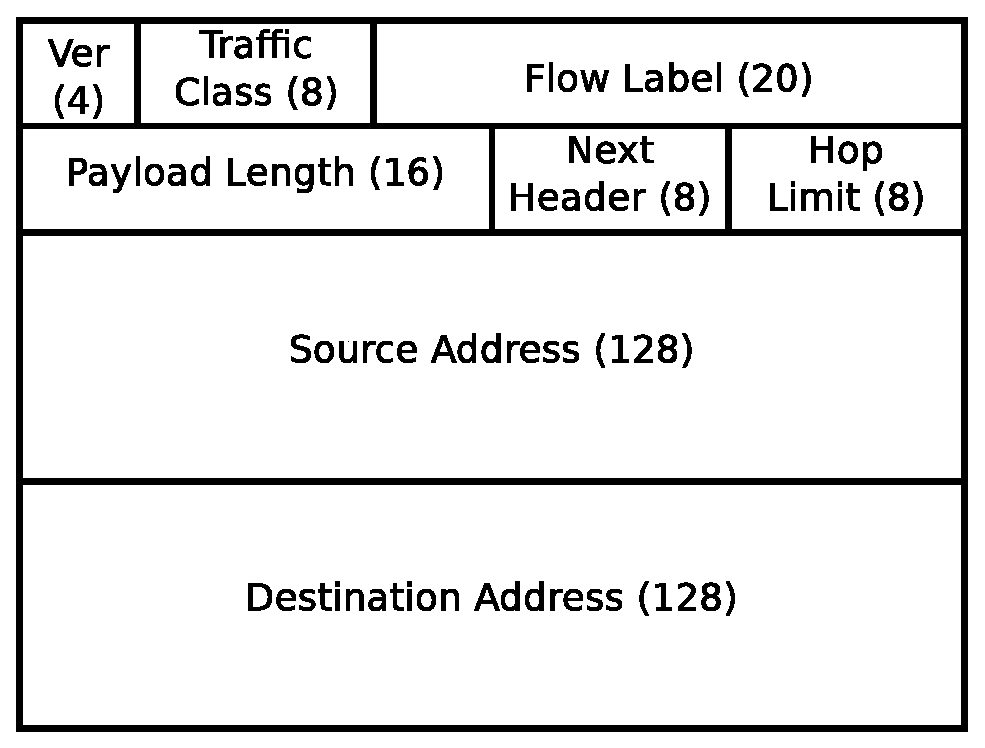
\includegraphics[width=4in]{IPv6_header}
% \caption{L'en-tête IPv6}
% \label{fig:IPv6}
% \end{figure}

% \begin{table}[htb]
% \caption{Plages de valeurs pour le champ \texttt{DSCP}}
% \centering
% \begin{tabular}{|c|c|l|}
% \hline\rowcolor[gray]{0.8}\color{black}
% Plage & Valeurs & Règle d'assignation\\\hline
% 1 & xxxxx0 & Assignation par une norme de l'IANA\\\hline
% 2 & xxxx11 & Expérimentation/Usage local\\\hline
% 3 & xxxx01 & Expérimentation/Usage local (pourrait être jointe à la plage 1)\\\hline
% \end{tabular}
% \label{tab:RangesDSCP}
% \end{table}

% % On veut éviter que la figure et le tableau soient placés au-delà de la section courante.
% % To prevent the figure and table from being positioned outside of the current section. 
% \FloatBarrier


% %%
% %% OBJECTIFS DE RECHERCHE / RESEARCH OBJECTIVES
% %%
% \section{Objectifs de recherche}  % 0.5 page
% Les objectifs de la recherche sont de concevoir un algorithme $O(n)$.


% %%
% %% PLAN DU MEMOIRE / THESIS OUTLINE
% %%
% \section{Plan du mémoire}  % 0.5 page

% Voir la Figure~\ref{fig:Layers} pour plus de détails. 

% \begin{figure}[htb]
% \centering
% 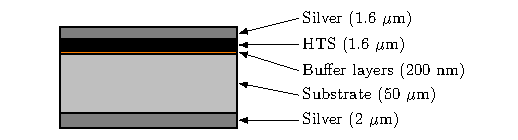
\includegraphics[width=4in]{demo_tikz}
% \caption{Couches}
% \label{fig:Layers}
% \end{figure}


% Un tableau : / A table:
% \begin{table}[htb]
%   \centering
%   \caption{Constantes et variables du modèle analytique}
%   \begin{tabular}{|c|l|}
%     \hline\rowcolor[gray]{0.8}\color{black}
%     Symbole         & Description\\\hline
%     $\lambda$       & Taux d'arrivée moyen des requêtes de réservation de ressources\\\hline
%     $\frac{1}{\mu}$ & Durée moyenne d'une session\\\hline
%     $C$             & Capacité d'une cellule (nombre de sessions supportées)\\\hline
%     $v_{moy}$       & Vitesse moyenne des MN dans le réseau d'accès\\\hline
%     $L$             & Longueur d'un côté d'une cellule carrée\\\hline
%     $n$             & Nombre moyen de MN dans une cellule\\\hline
%     $\rho$          & Charge d'une cellule\\\hline
%     $P_b$           & Probabilité de blocage d'une requête de réservation\\\hline
%     $P_f$           & Probabilité d'interruption forcée d'une session\\\hline
%     $P_c$           & Probabilité de compléter une session avec succès\\\hline
%     $\Delta{}T$     & Délai de transmission\\\hline
%   \end{tabular}
%   \label{tab:Definitions}
% \end{table}

% La formule d'\mbox{Erlang-B}:
% \begin{equation}
%   P_b = \frac{\frac{\rho^C}{C!}}{\sum\limits_{x=0}^{C}\frac{\rho^x}{x!}}
%   \label{eq:Pblock}
% \end{equation}

% Une autre équation : / Another equation:
% \begin{equation}
%   \begin{split}
%     P_c &= (1 - P_b) \times (1 -  P_f)^N\\
%         &= (1 - P_b)^{N+1}
%   \end{split}
%   \label{eq:ProbComplete}
% \end{equation}

% Enfin, l'expression suivante indique le moment à partir duquel les
% réservations de ressources sont en place:
% \begin{equation}
%   \Delta{}T_{init} =
%   \begin{cases}
%     2\Delta{}T_{E2E} & \Delta{}T_{wan} > (\Delta{}T_{rad} + \Delta{}T_{net})\\
%     \Delta{}T_{E2E} + 3(\Delta{}T_{rad} + \Delta{}T_{net}) & \text{sinon}
%   \end{cases}
%   \label{eq:InitCost}
% \end{equation}

% \paragraph{Le taux de paquets perdus} correspond au nombre de paquets
% éliminés à cause d'une erreur de \emph{checksum} à un n\oe{}ud
% quelconque ou d'une situation de congestion. Le taux de paquets perdus
% pour un chemin est déterminé de la façon suivante:
% \begin{equation}
%   \label{eq:genPLR}
%   PLR_P = 1 - \prod_{i=1}^N(1 - PLR_i)
% \end{equation}

% Toutefois, si les taux d'erreurs sont très faibles, comme c'est
% généralement le cas pour des liens optiques, on peut approximer
% $PLR_P$ de façon à le transformer en un paramètre additif:
% \begin{equation}
%   \label{eq:approxPLR}
%   \begin{split}
%     PLR_{L_1 \oplus L_2} &= 1 - (1 - PLR_1)(1 - PLR_2)\\
%     &= 1 - (1 - PLR_2 - PLR_1 + \underbrace{PLR_1
%       \times PLR_2}_\text{négligeable})\qquad PLR_1 \ll 1,
%     PLR_2 \ll 1\\
%     &\approx PLR_1 + PLR_2
%   \end{split}
% \end{equation}

% \clearpage

% Une courbe : / A curve:
% \begin{figure}[htb]
% \centering
% 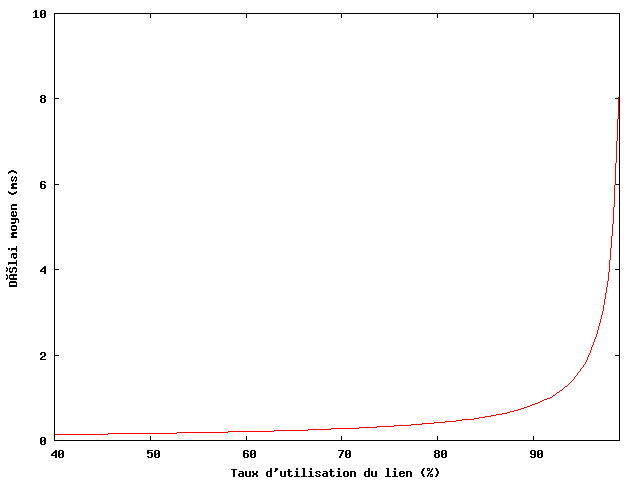
\includegraphics[width=5in]{LinkUsage}
% \caption{Délai moyen en fonction du taux d'utilisation d'un lien}
% \label{fig:LinkUse}
% \end{figure}

% \selectlanguage{english}
% This paragraph is formatted by \LaTeX{} according to the standard rules of the
% English language (\mbox{e.g.} hyphenation).
% \selectlanguage{french}

% L'arithmétique en virgule flottante peut entraîner des erreurs
% d'approximation et il est important d'en être conscient
% \cite{Rossi2011}.

% De même, les calculs effectués sur une carte graphique (GPU) peuvent
% introduire des erreurs d'approximation \cite{DeSantis2002, Cohen2006,
%   Thorsson2014, Schirmer2012, Sakai2015, Electrical2006,
%   Min2016, Massicotte2013, Kaliouby1987, Daintith2010, Haist2014, Kizza2013,
%   Manasreh2011, Brydson1999, Boyce2002}.
